\documentclass[11pt]{article}
\usepackage[utf8]{inputenc}
\usepackage{scalefnt}
\usepackage{lmodern} 
\usepackage{amsfonts, amsmath}
\usepackage{graphicx, caption, subcaption} % Graphics
\usepackage{float} % Graphics using H
\usepackage[letterpaper, margin=1in]{geometry}

\usepackage{color}
\newcommand{\FIXME}[1]{ \ \\ \hspace* {-1.5 cm}
  \textcolor{red}{\texttt{FIXME:}#1} \medskip\par}


\begin{document}

\begin{titlepage}

\centering
	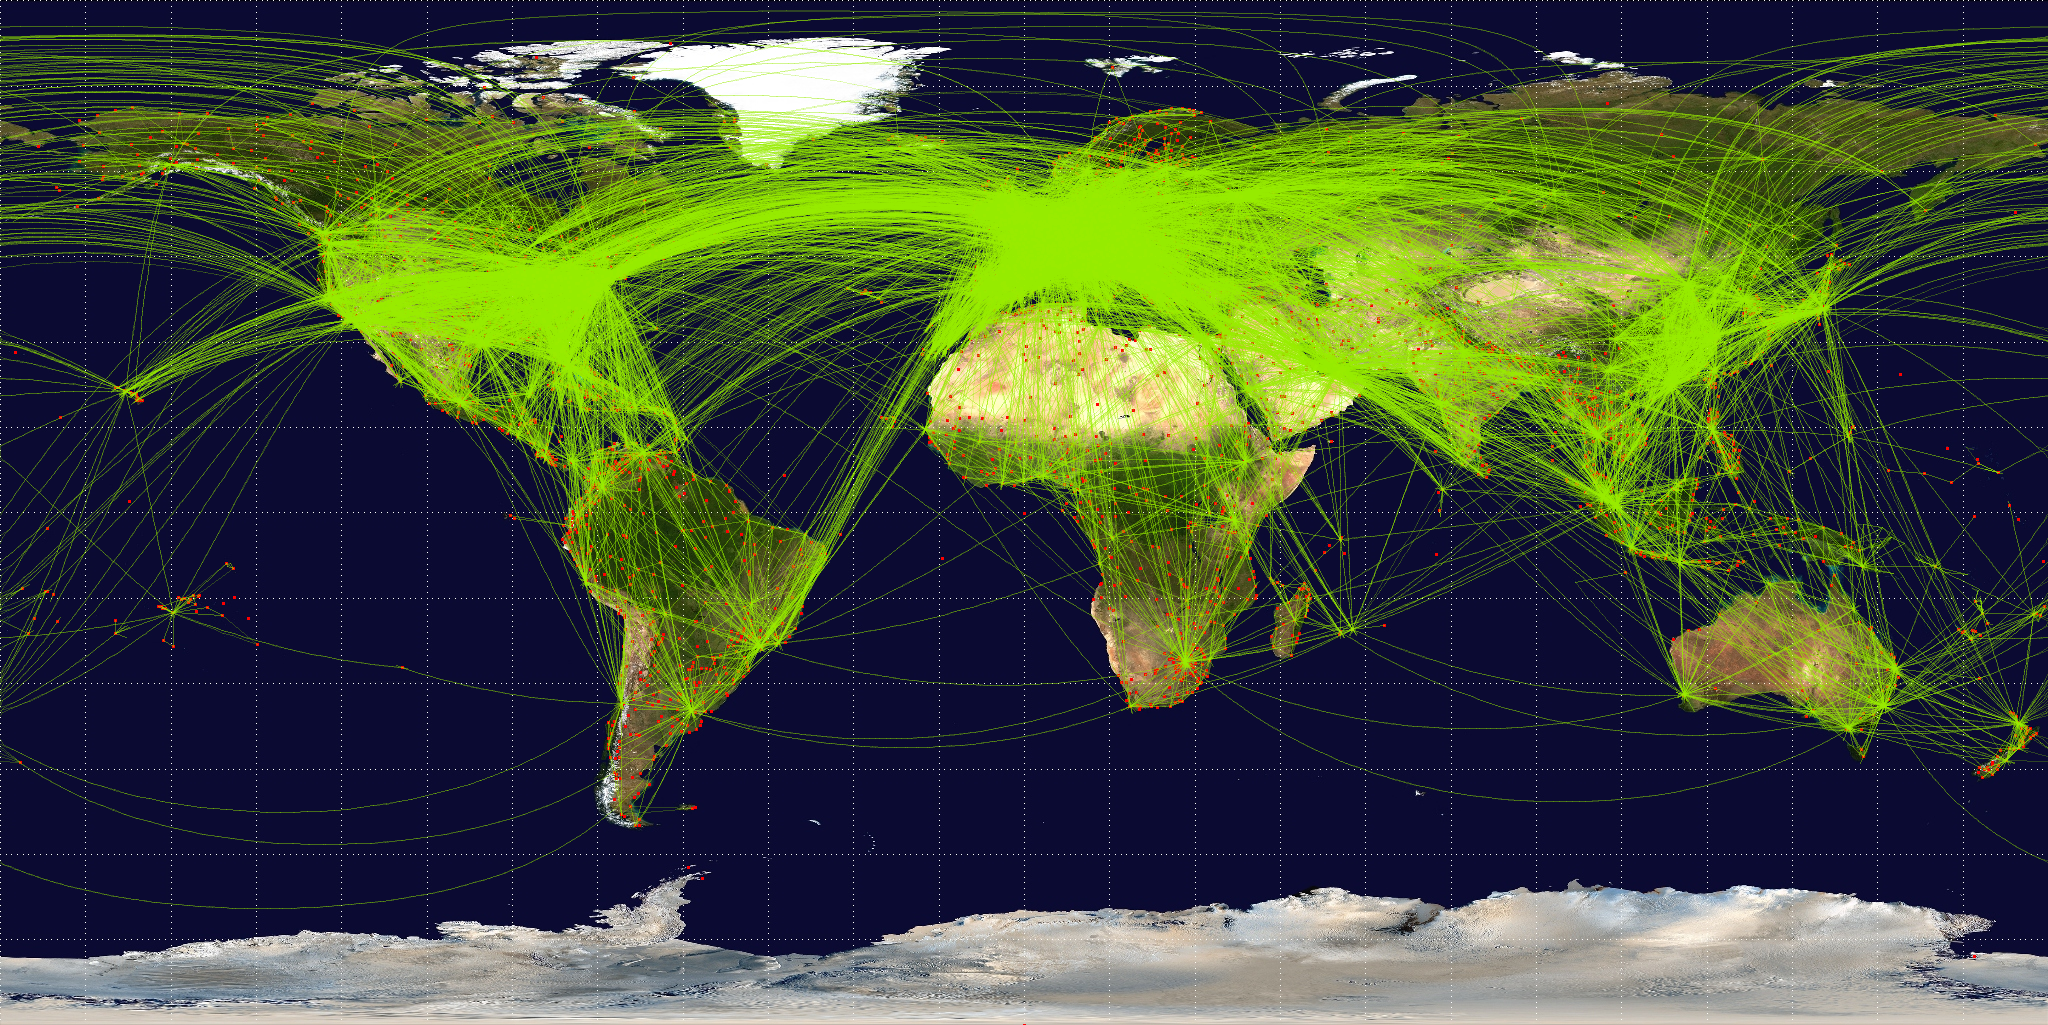
\includegraphics[width=0.5\textwidth]{map}\par\vspace{1cm}
	{\scshape\LARGE  \par}
	\vspace{1cm}
	{\scshape\Large Project Report \par}
	\vspace{1.5cm}
	{\huge\bfseries Minimal Time Paths \par}
	\vspace{2cm}
	{\Large\itshape Alex Dunkel,
Roy Gullem,
Keith Houpy, \\
Emily Ribando-Gros, and
Vincent Rodomista\par}
	\vfill
	\textsc{CSC 4444}

	\vfill

% Bottom of the page
	{\large \today\par}
\end{titlepage}

\tableofcontents

\pagebreak

\section{Motivation}

Travel plans can be extremely complicated. As a college student, when planning a trip, you can sift through numerous flights looking for deals and also weigh the cost of driving based on gas prices and car mileage. On the other hand, a business person may do the same sort of sifting to find the fastest, most direct flights and available private transportation in order to get to their destination as fast as possible without considering the price. We are given many options when considering travel plans, and planning could end up in a series of calculations based on time, price of travel, or both. 

\section{Problem}
We want to find the path from one point to another by minimizing time or price by either driving, flying, or a combination of both. To ensure that the price of this path is not too high, we can specify a price limit so that we find the fastest path under that price limit.

\subsection{Problem Formulation}
\begin{enumerate}
\item \textbf{Initial State}: The user's starting point
\item \textbf{States}: contact points
%\item \textbf{State Space}: All possible contact points
\item	 \textbf{Actions}: either fly or drive to a destination. For example, Drive(\emph{destination}) or Fly(\emph{destination})
%\item	 \textbf{Actions}: The modes of transportation used between two contact points, either drive or fly
\item \textbf{Transition Model}: given a state and action moves the user to the new contact point
\item \textbf{Goal State}: the user's destination
\item \textbf{Path}: a sequence of actions from the initial state to the goal state
\item \textbf{Path Costs}: the time or price it takes to get from one contact point to another % and a heuristic component
\item \textbf{Solution}: the path from the initial state to the goal state that does not exceed the price limit
\end{enumerate}

\section{AI Concepts}
\subsection{Search Tree}

\subsubsection{Node} A Node in the search tree represents a contact point along the path. Node attributes include
\begin{itemize}
\item State : Information about the contact point such as a name and latitude longitude coordinates
\item Parent : The node in the search tree which generated this node
\item Action : The action (fly or drive) applied to the parent to generate this node
\item Path costs in time and price : the time and price needed to travel from the initial node to the current node
\end{itemize}

\subsubsection{Frontier}

After expanding a leaf node in our search tree, the general search tree algorithm collects the next set of available leaf nodes for expansion in the frontier. But before searching can continue, our algorithm must check whether any of the frontier nodes will result in a path cost price which exceeds the user's price limit. In other words, if the price of a path exceeds the given price limit we do not add the next node to the frontier. This way we can ensure that we never find a path with a price that is above the limit. Nodes are selected for expansion based on the search strategies described in \ref{sec:search}.

\subsection{Constraints}

\subsubsection{Branching Factor}

When searching for a path, given the number of airports and cities in the US, our branching factor could be very large. Because of this, some constraints must be considered. Let $A$ be the initial starting point and let $B$ be the destination point. We limit the number of airports around $A$, say $\{ A_i \}_{i=1}^n$, and the number of airports around the destination point, say $\{ B_j \}_{j=1}^m$. The agent can then drive from $A$ to one of the airports in $\{ A_i \}_{i=1}^n$ or drive directly to $B$. If the agent is at one of the airports in $\{ A_i \}_{i=1}^n$, the only option for the agent is to fly to one of the airports in $\{ B_j \}_{j=1}^m$. If the agent is at an airport around $B$, then the only possible action is to drive to the destination $B$. Figure~\ref{fig:graph_example} shows an example with a graph with $n = 2$ and $m = 2$.
\begin{figure}[!ht]
  \caption{Graph example with $n=2$ and $m=2$.}
  \centering
  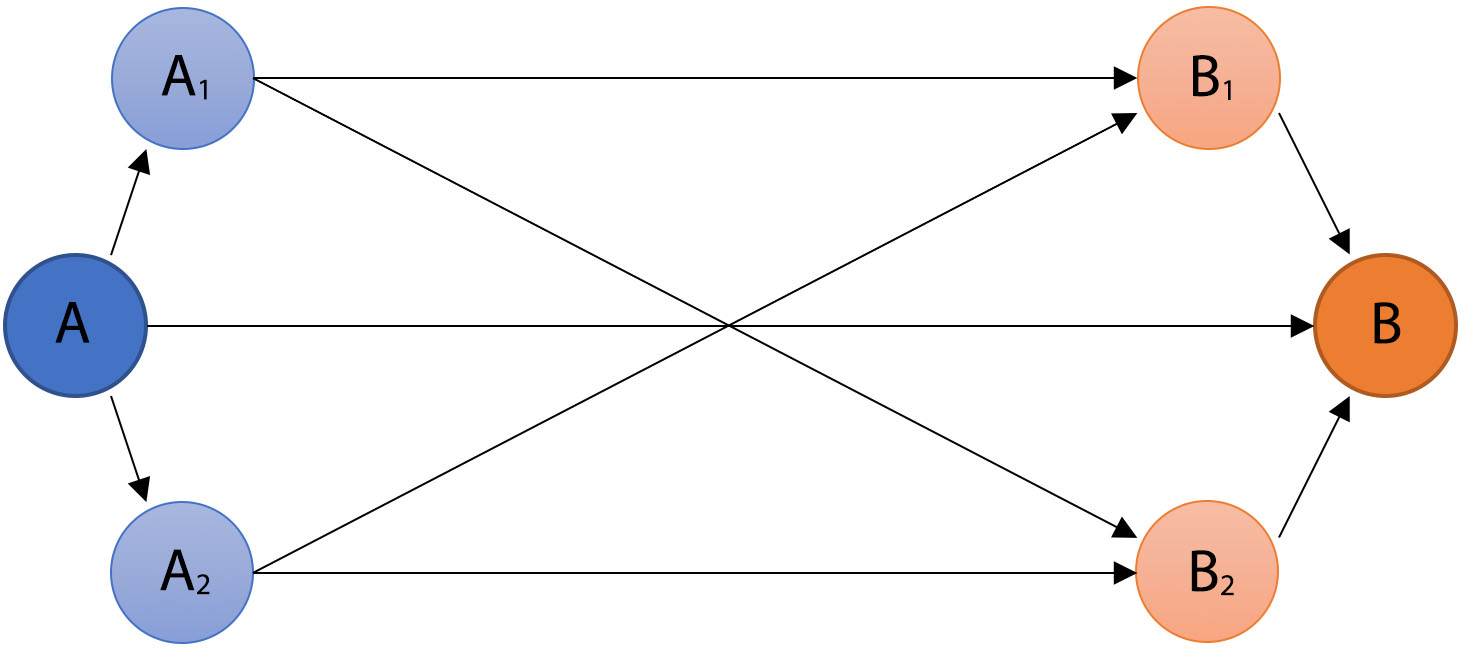
\includegraphics[width=0.8\textwidth]{Graph_example_n2}
  \label{fig:graph_example}
\end{figure}

\subsubsection{Driving Assumptions}

In order to calculate driving time and cost, a few assumptions were hard coded into our application. To give a more accurate description of the time it takes to drive across the country, every 12 hours we will assume that our user will spend \$75 on a hotel. We will add this price to our path price when searching for a solution. Similarly, when calculating time we will only assume that the user will drive 12 hours a day. In other words, for every 12 hours of driving, a cost of \$75 is added to the path price and 12 hours are added to the path time. Additionally, we assumed that a car has 35 miles per gallon and a gallon of gas is \$2.15.
These assumptions can be seen in \ref{fig:drivuml}.


\section{Search Strategies and Experimentation}\label{sec:search}

\subsection{Uniform Cost Search}

At the base line, our algorithm performs a tree search seeking to minimize the time it takes to travel given a price limit. 
Since different users may value their time more than their money or may not like driving, we considered the following features.

\subsubsection{UCS Experiment : Amite, LA to Stockton, CA and Hayward, CA}

The following searches were done without a price limit and with a price limit of \$250. At the very bottom of the tree, there is one node to represent the driving distance, which ends up being more expensive then either of the flights we found. 

\subsubsection{Minimum time with minimum price flights}\label{sec:sol}

In the first search, we used UCS minimizing time without a price limit. When choosing flights between two places, we chose the minimum priced flight.

\begin{center}
Solution : Amite $\rightarrow$ MSY(1.2 hr) $\rightarrow$ LAX1(4.4 hr) $\rightarrow$ Stockton(5.2 hr) \\
\quad Total Price: \$255 \\
\quad Total Time: 10 hrs and 48 min
\end{center}

\begin{figure}[!ht]
  %\caption{Search when minimizing time without price limit.}
  \centering
  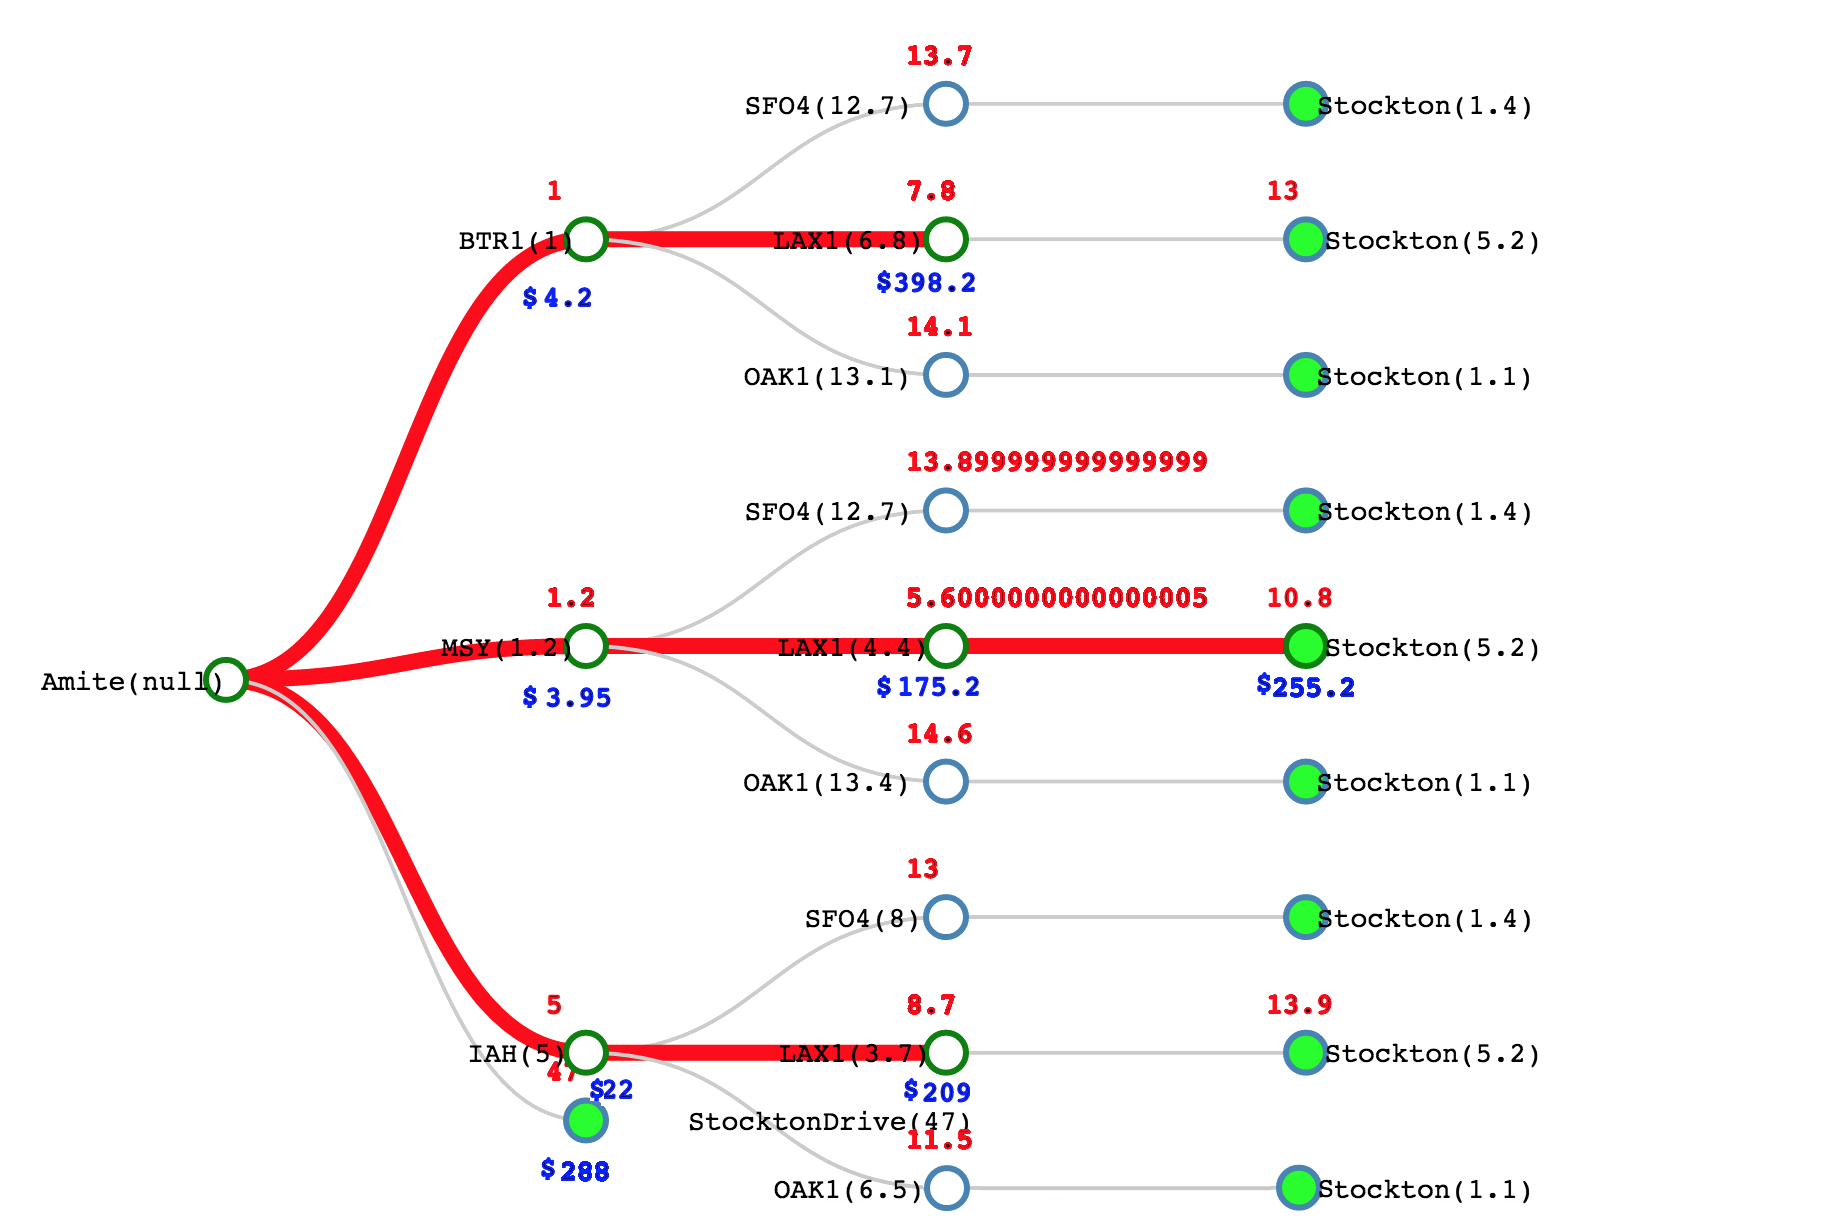
\includegraphics[width=0.8\textwidth]{time}
  \label{fig:time}
\end{figure}

\pagebreak

\subsubsection{Minimum time with minimum price flights and limit}

In the second search, we used UCS minimizing time with a price limit of \$250. When choosing flights between two places, we chose the minimum priced flight.

\begin{center}
Solution : Amite $\rightarrow$ IAH(5 hr) $\rightarrow$ LAX1(3.7 hr) $\rightarrow$ Stockton(5.2 hr) \\
\quad Total Price: \$230 \\
\quad Total Time: 13 hrs and 54 min\\
\end{center}

\begin{figure}[!ht]
  \centering
  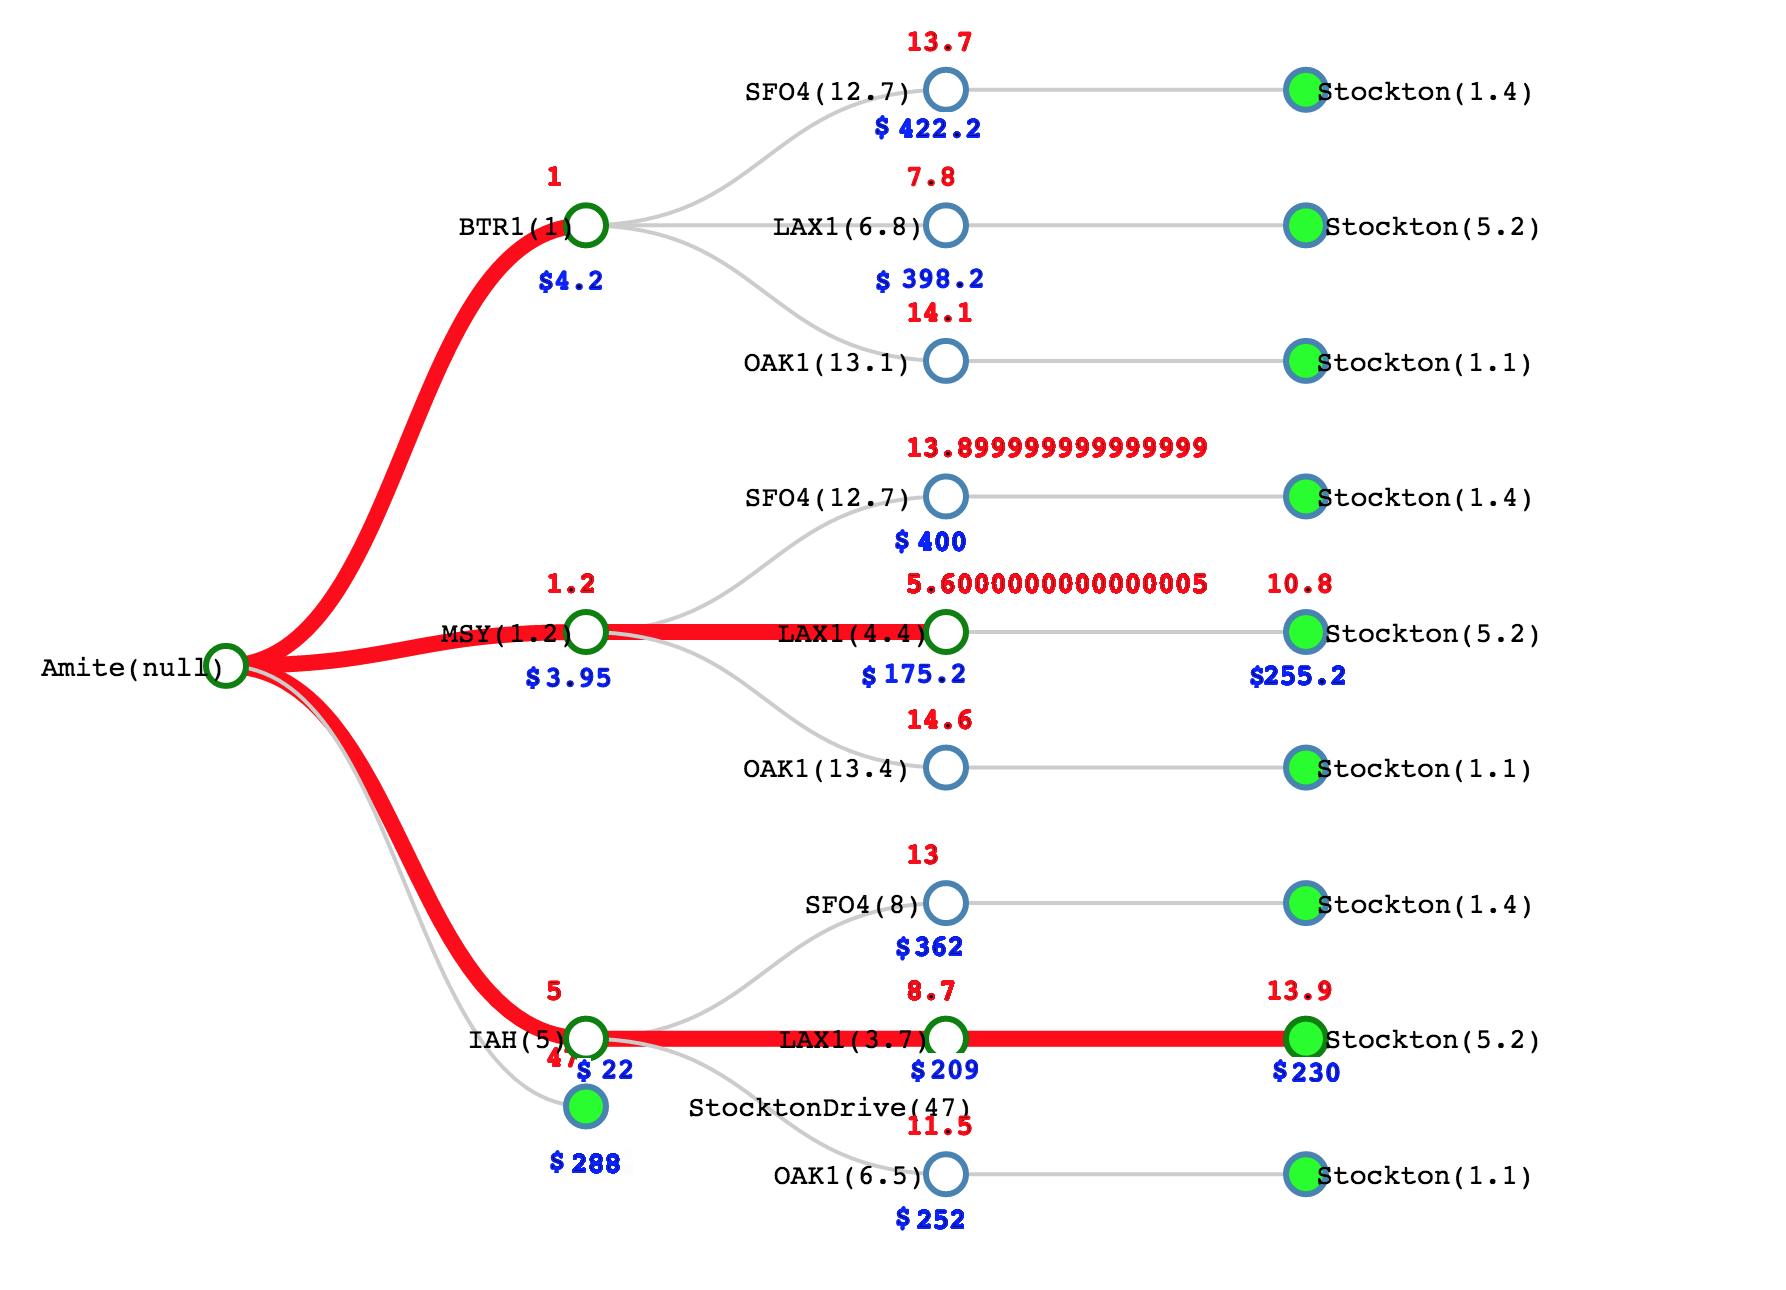
\includegraphics[width=0.8\textwidth]{time_lim}
  %\caption{Search when minimizing time with price limit of \$250.}
  \label{fig:time_lim}
\end{figure}

\pagebreak

\subsubsection{Minimum time with minimum time flights}

In the third search, we used UCS minimizing time. When choosing flights between two places, we chose the minimum priced flight.

\begin{center}
Solution : Amite  $\rightarrow$ Hayward \\
\quad Total Price: \$530 \\
\quad Total Time: 6 hrs 23 min\\
\end{center}

\subsubsection{Minimum price with minimum price flights}

In the fourth search, we used UCS minimizing price. When choosing flights between two places, we chose the minimum priced flight.

\begin{center}
Solution : Amite $\rightarrow$ Hayward \\
\quad Total Price: \$287 \\
\quad Total Time: 31 hrs and 24 min\\
\end{center}

\begin{figure}[!ht]
  \centering
  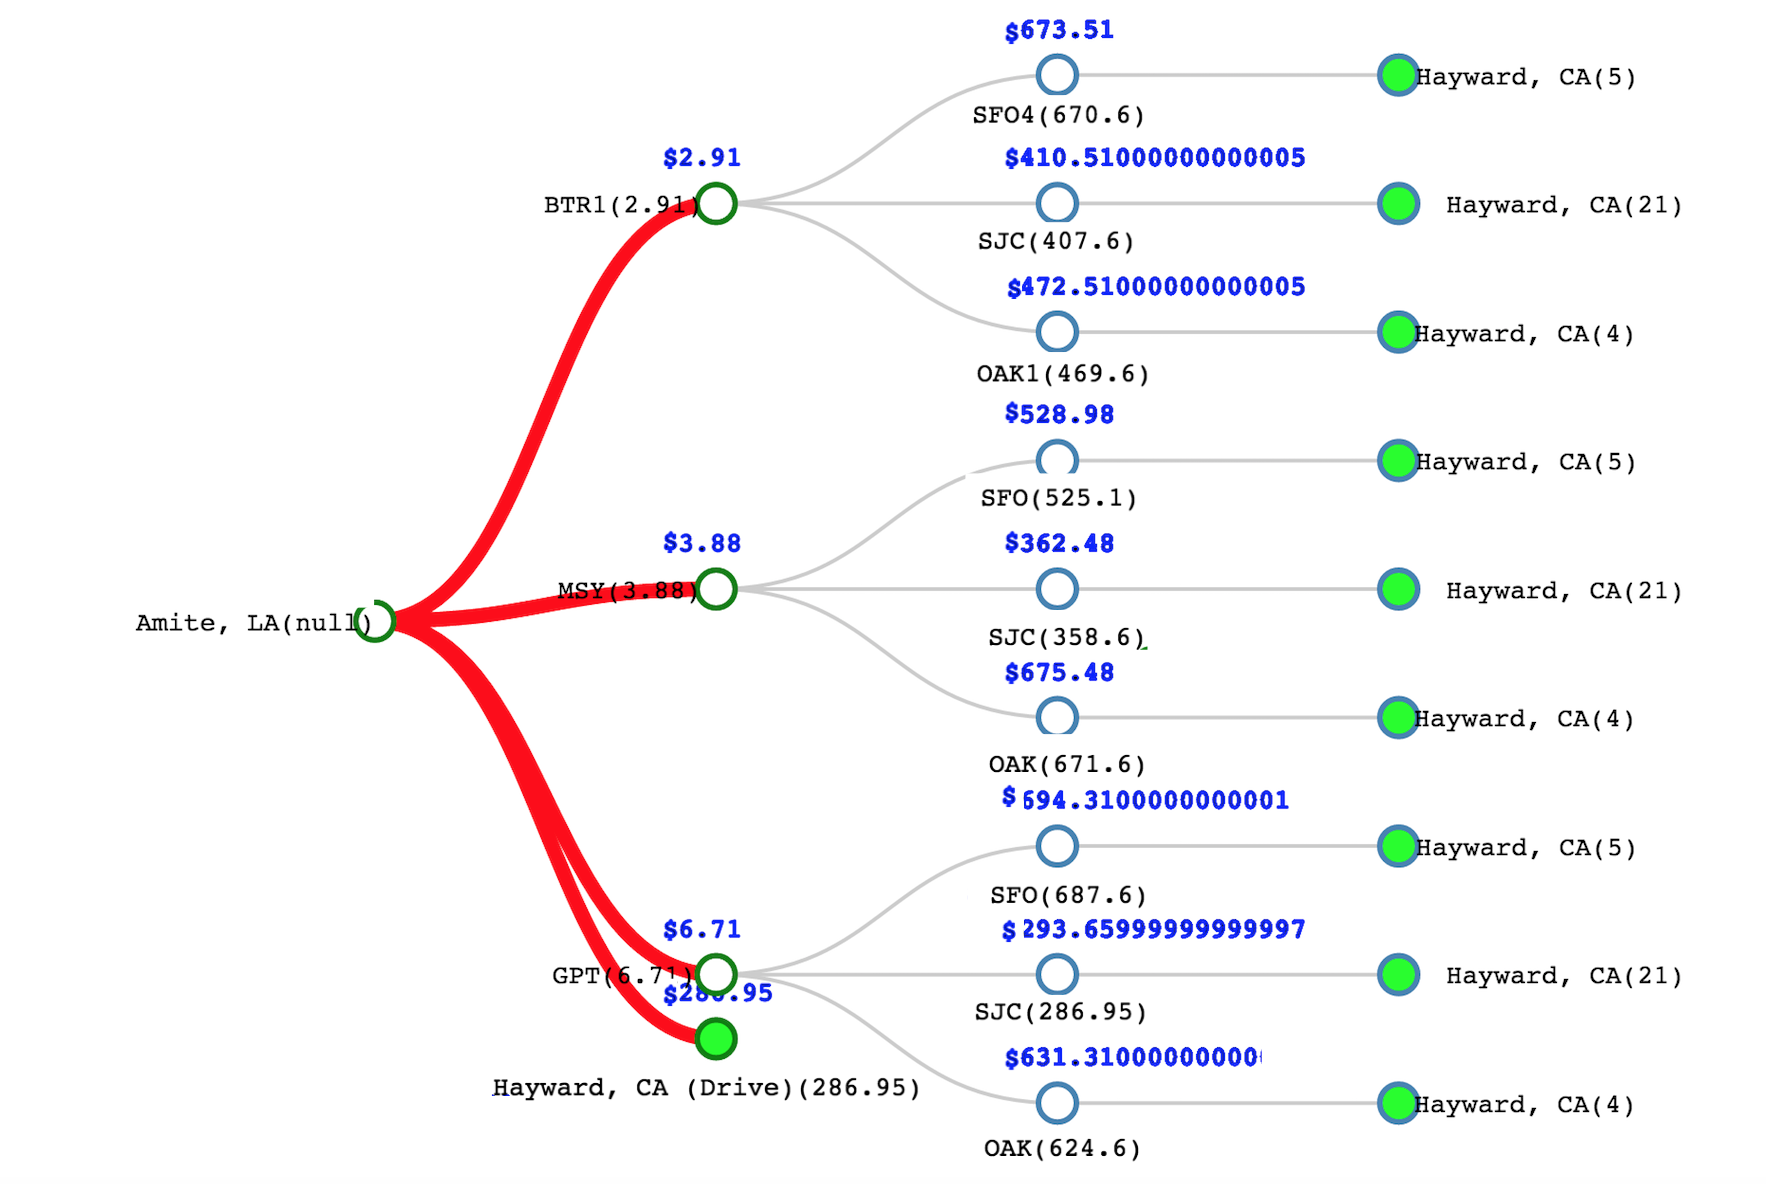
\includegraphics[width=0.8\textwidth]{price}
  %\caption{Search when minimizing time with price limit of \$250.}
  \label{fig:tprice}
\end{figure}

\pagebreak

\subsection{A* Search with Straight Line Heuristic}

In addition to the above features, we thought that we could improve upon our algorithm by adding a heuristic component to our cost function. 
Across edges, we are mixing different modes of transportation which have different speeds. Additionally, costs for flying depends only on plane tickets where as costs for driving depends directly on the distance and miles per gallon of a vehicle. 
For this reason, we can not simply just use the distance as a heuristic but we need to first convert it to the proper units based on what we would like to minimize.

\subsubsection{A* Experiment : Estimating Time based on Distance}

Since commercial flights do not reach a speed faster than 600 mph, we tested adding the distance between two places divided by this speed. 
We found distance using the Haversine formula. If the latitude and longitude of a node $n$ and the destination are $(\phi_1,\phi_2)$ and $(\lambda_1,\lambda_2)$ and r is the radius of the earth then,

$$d = 2r \arcsin \left( \sqrt{\sin^2 \left(\frac{\phi_2-\phi_1}{2} \right)+\cos(\phi_2) \cos(\phi_2) \sin^2 \left( \frac{\lambda_2 - \lambda_1}{2} \right)} \right)$$

We then let
$$h(n) = \frac{d}{600} \text{ hours }$$

Using the previous example, we calculated the following costs for $h(n)$.

\begin{figure}[!ht]
  \centering
  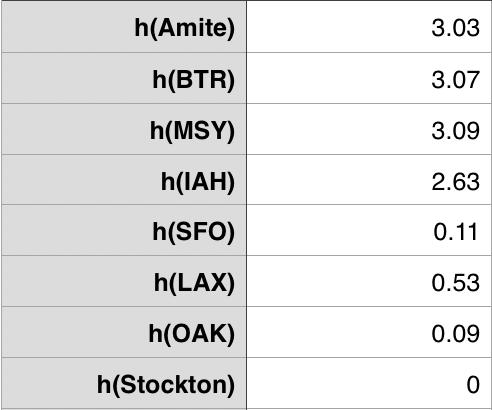
\includegraphics[width=0.35\textwidth]{hn}
  %\caption{Search when minimizing time with price limit of \$250.}
  \label{fig:time_lim}
\end{figure}

In the end, we arrived at the same solution from \ref{sec:sol}.

\subsubsection{Conclusion}

When we use a heuristic based on the straight line distance, nodes that are closer to the goal node are more likely to get chosen. We noticed that this heuristic did not improve the performance. Suppose we want to go from $A$ to $B$. There are two airports around $A$ that have the same distance to $A$. One of the airports, say $A_1$, is a small airport that lies along the way from $A$ to $B$. The other airport, say $A_2$, is a large airports that is out of the way. With this heuristic $A_1$ would get selected first. Since $A_1$ is a small airport, it does not have a direct flight towards the goal node. Having a layover would add a lot of time. The airport $A_2$, on the other hand, does have a direct flight. Thus, it would be better to select $A_2$ first. 

\section{Software System Design and Implementation}

We chose to use Java for our project in the IDE IntelliJ. We developed our GUI in JavaFX using the JFoenix design library.
To compute the time and price of each edge we use many different Google APIs. 

\subsection{Search Classes}

Given the latitude and longitude of the initial point (origin) and destination (goal), our search algorithm uses a few different classes to arrive at a solution.
In \ref{fig:suml} you can see the relevant fields and methods for each class.
\begin{enumerate}
\item \texttt{Problem.java} : stores information about the travel plans of the user 
\item \texttt{Node.java} : represents a node in the search tree
\item \texttt{Search.java} : search algorithm logic
\item \texttt{FindAirports.java} : finds the n airports around a place
\end{enumerate}

\begin{figure}[!ht]
  \centering
  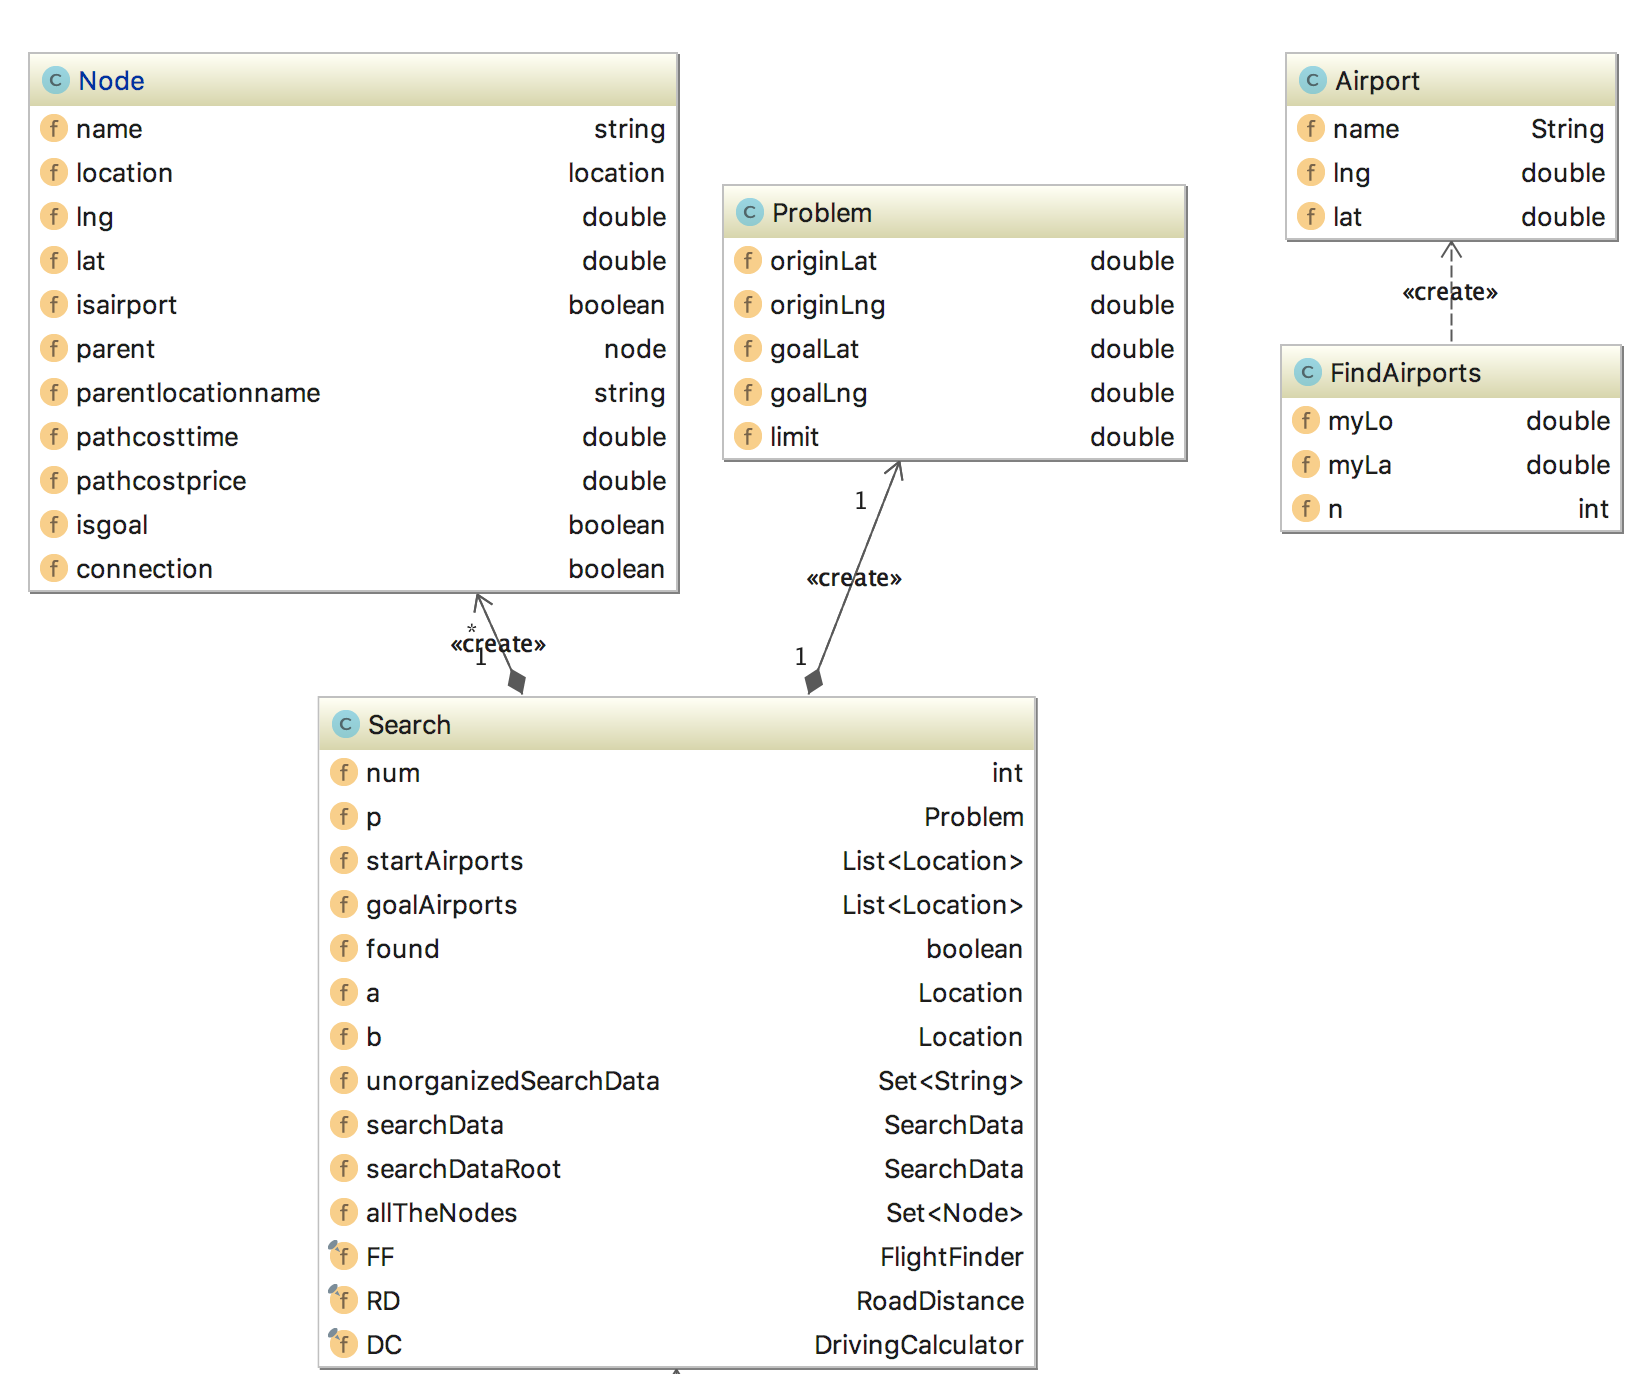
\includegraphics[width=0.8\textwidth]{searchuml.png}
  \caption{Search Classes}
  \label{fig:suml}
\end{figure}

\pagebreak

\subsection{Map Utilities}

\subsubsection{Road Distance and Driving Calculator }

\texttt{RoadDistance.java} gives simple distance, and driving time between two places (no driving
directions though); a place can be coordinates, a zip, an address, or any string that would turn up a result in Google Maps. Uses Google Maps
Distance Matrix API. \\
Main methods are: 
\begin{itemize}
\item \texttt{getRoadDistance(String, String)}
\item \texttt{getRoadTime(String, String)}
\item \texttt{getRoadDistance(Location, Location)}
\item \texttt{getRoadTime(Location, Location)}
\end{itemize}

\texttt{DrivingCalculator.java} figures out total price (gas + hotel) and duration (driving plus sleep) of a road trip. Main inputs are miles and hours (which you can get from
 \texttt{RoadDistance.java}).\\
 Key constructor:
 \begin{itemize}
 \item  \texttt{DrivingCalculator(double, double)}
 \end{itemize}
  Key methods:
  \begin{itemize}
\item  \texttt{calc()},
 \item  \texttt{calc(double, double)}
 \end{itemize}

\begin{figure}
\centering
\begin{subfigure}{.4\textwidth}
\centering
  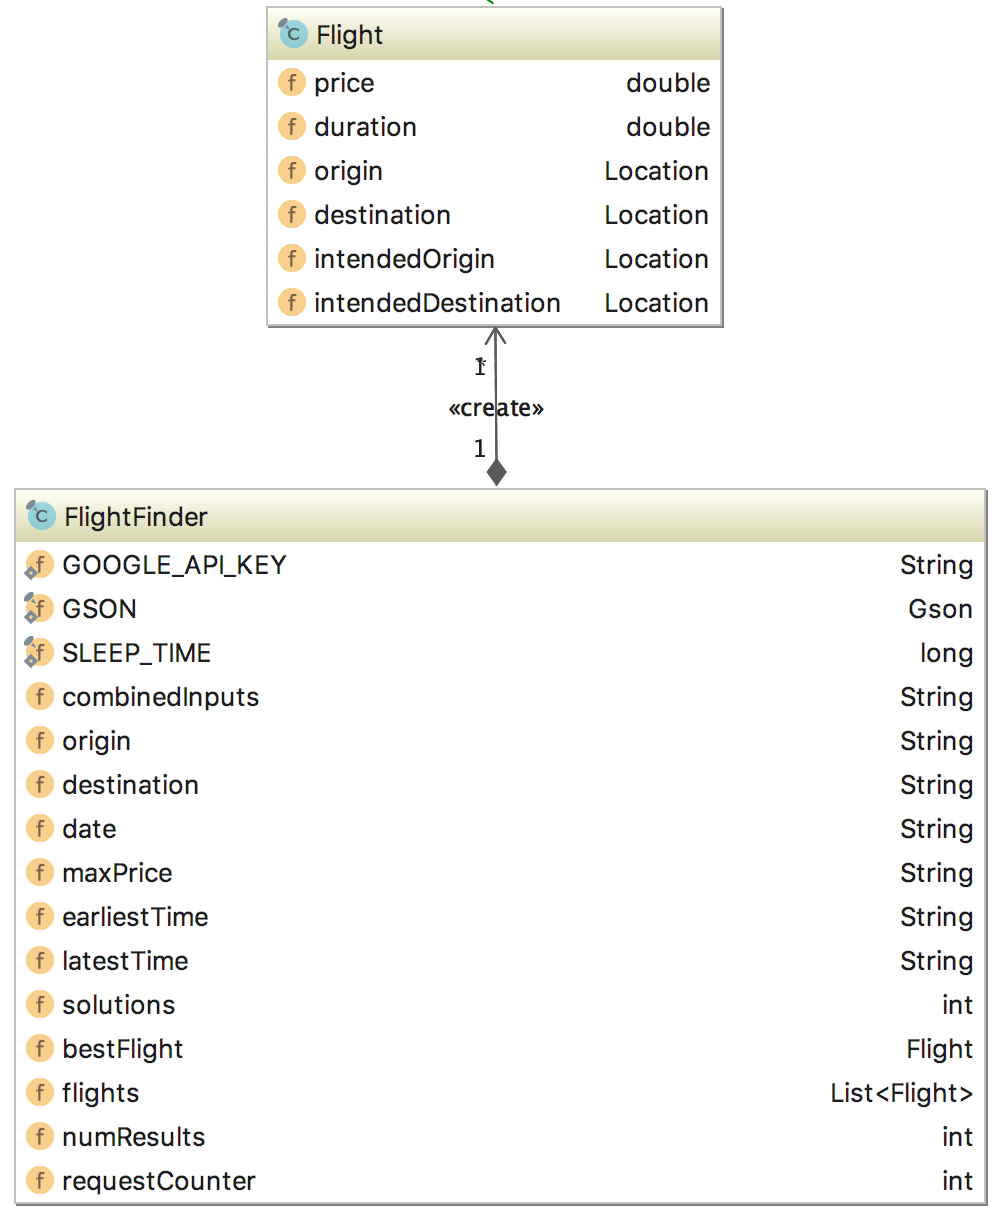
\includegraphics[width=1\linewidth]{FlightFinder.png}
  \caption{Flight Finder}
  \label{fig:flfinder}
\end{subfigure}%
\begin{subfigure}{.6\textwidth}
\centering
  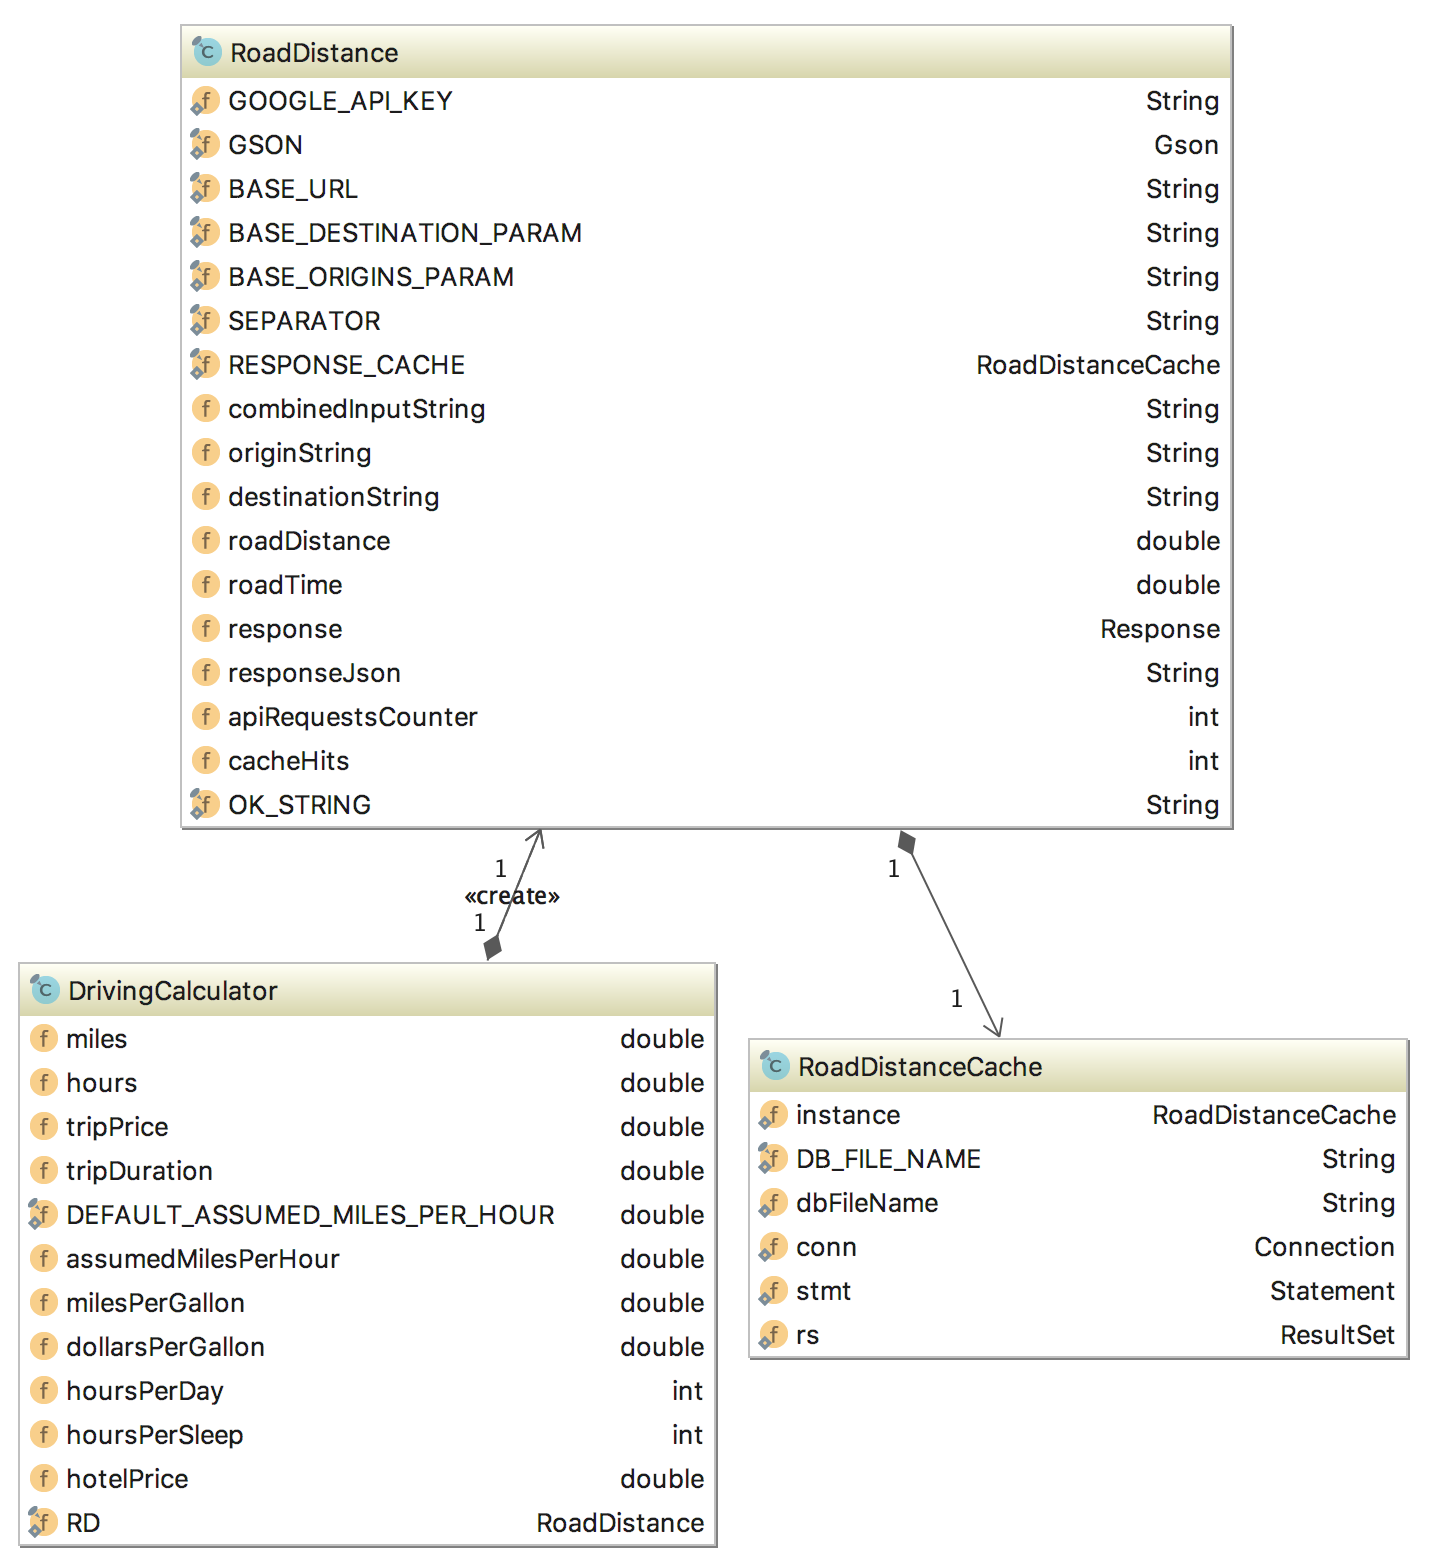
\includegraphics[width=1.1\linewidth]{driveuml}
  \caption{Driving Utilities}
  \label{fig:drivuml}
\end{subfigure}
\caption{Map Utilities}
\label{fig:util}
\end{figure}

\subsection{APIs}

To gather data, we chose Google APIs for their ease of use specifically using HTTP transport and JSON parsing features. 
Below are the following APIs used and how they were used.

\begin{itemize}
\item QPX Express Airfare API : flight finder
\item Google Maps Distance Matrix API : estimate travel time
\item Google Maps Geocoding API : convert between addresses and latitude/longitude coordinates
\item Google Maps Directions API : driving directions
\item Google Places API Web Service : places autocomplete
\end{itemize}


\pagebreak

\subsection{Caching}

Some of the APIs are quite slow, especially the QPX Express Airfare API to find flights. So to speed up our search time, we tried caching the data we found for future searches.
We use two separate caches to make searches faster. One cache is used for road travel and one for flight. When we call the function used to determine the best route, it first searches the cache to see if the query has already been made in the past. If it has, it returns the result of the query. If this data is not stored, the API is called and the resulting distance is stored in the cache. This speeds up searching significantly over time because the cache will be able to be referenced more, avoiding costly calls to the API. The API calls take significantly longer than the cache calls, so it becomes faster and faster over time. In Figure \ref{fig:db} you can see a view of the physical data in the schema. Initially, we thought to use Bluemix for our database. We tried to integrate Bluemix but ran into complications passing information onto their server. It ended up being much simpler to manage our data locally using our caches and calling the API when necessary. Given more times and resources, we would ideally integrate a Bluemix database into our project and analyze the data.

\begin{figure}[!ht]
  \centering
  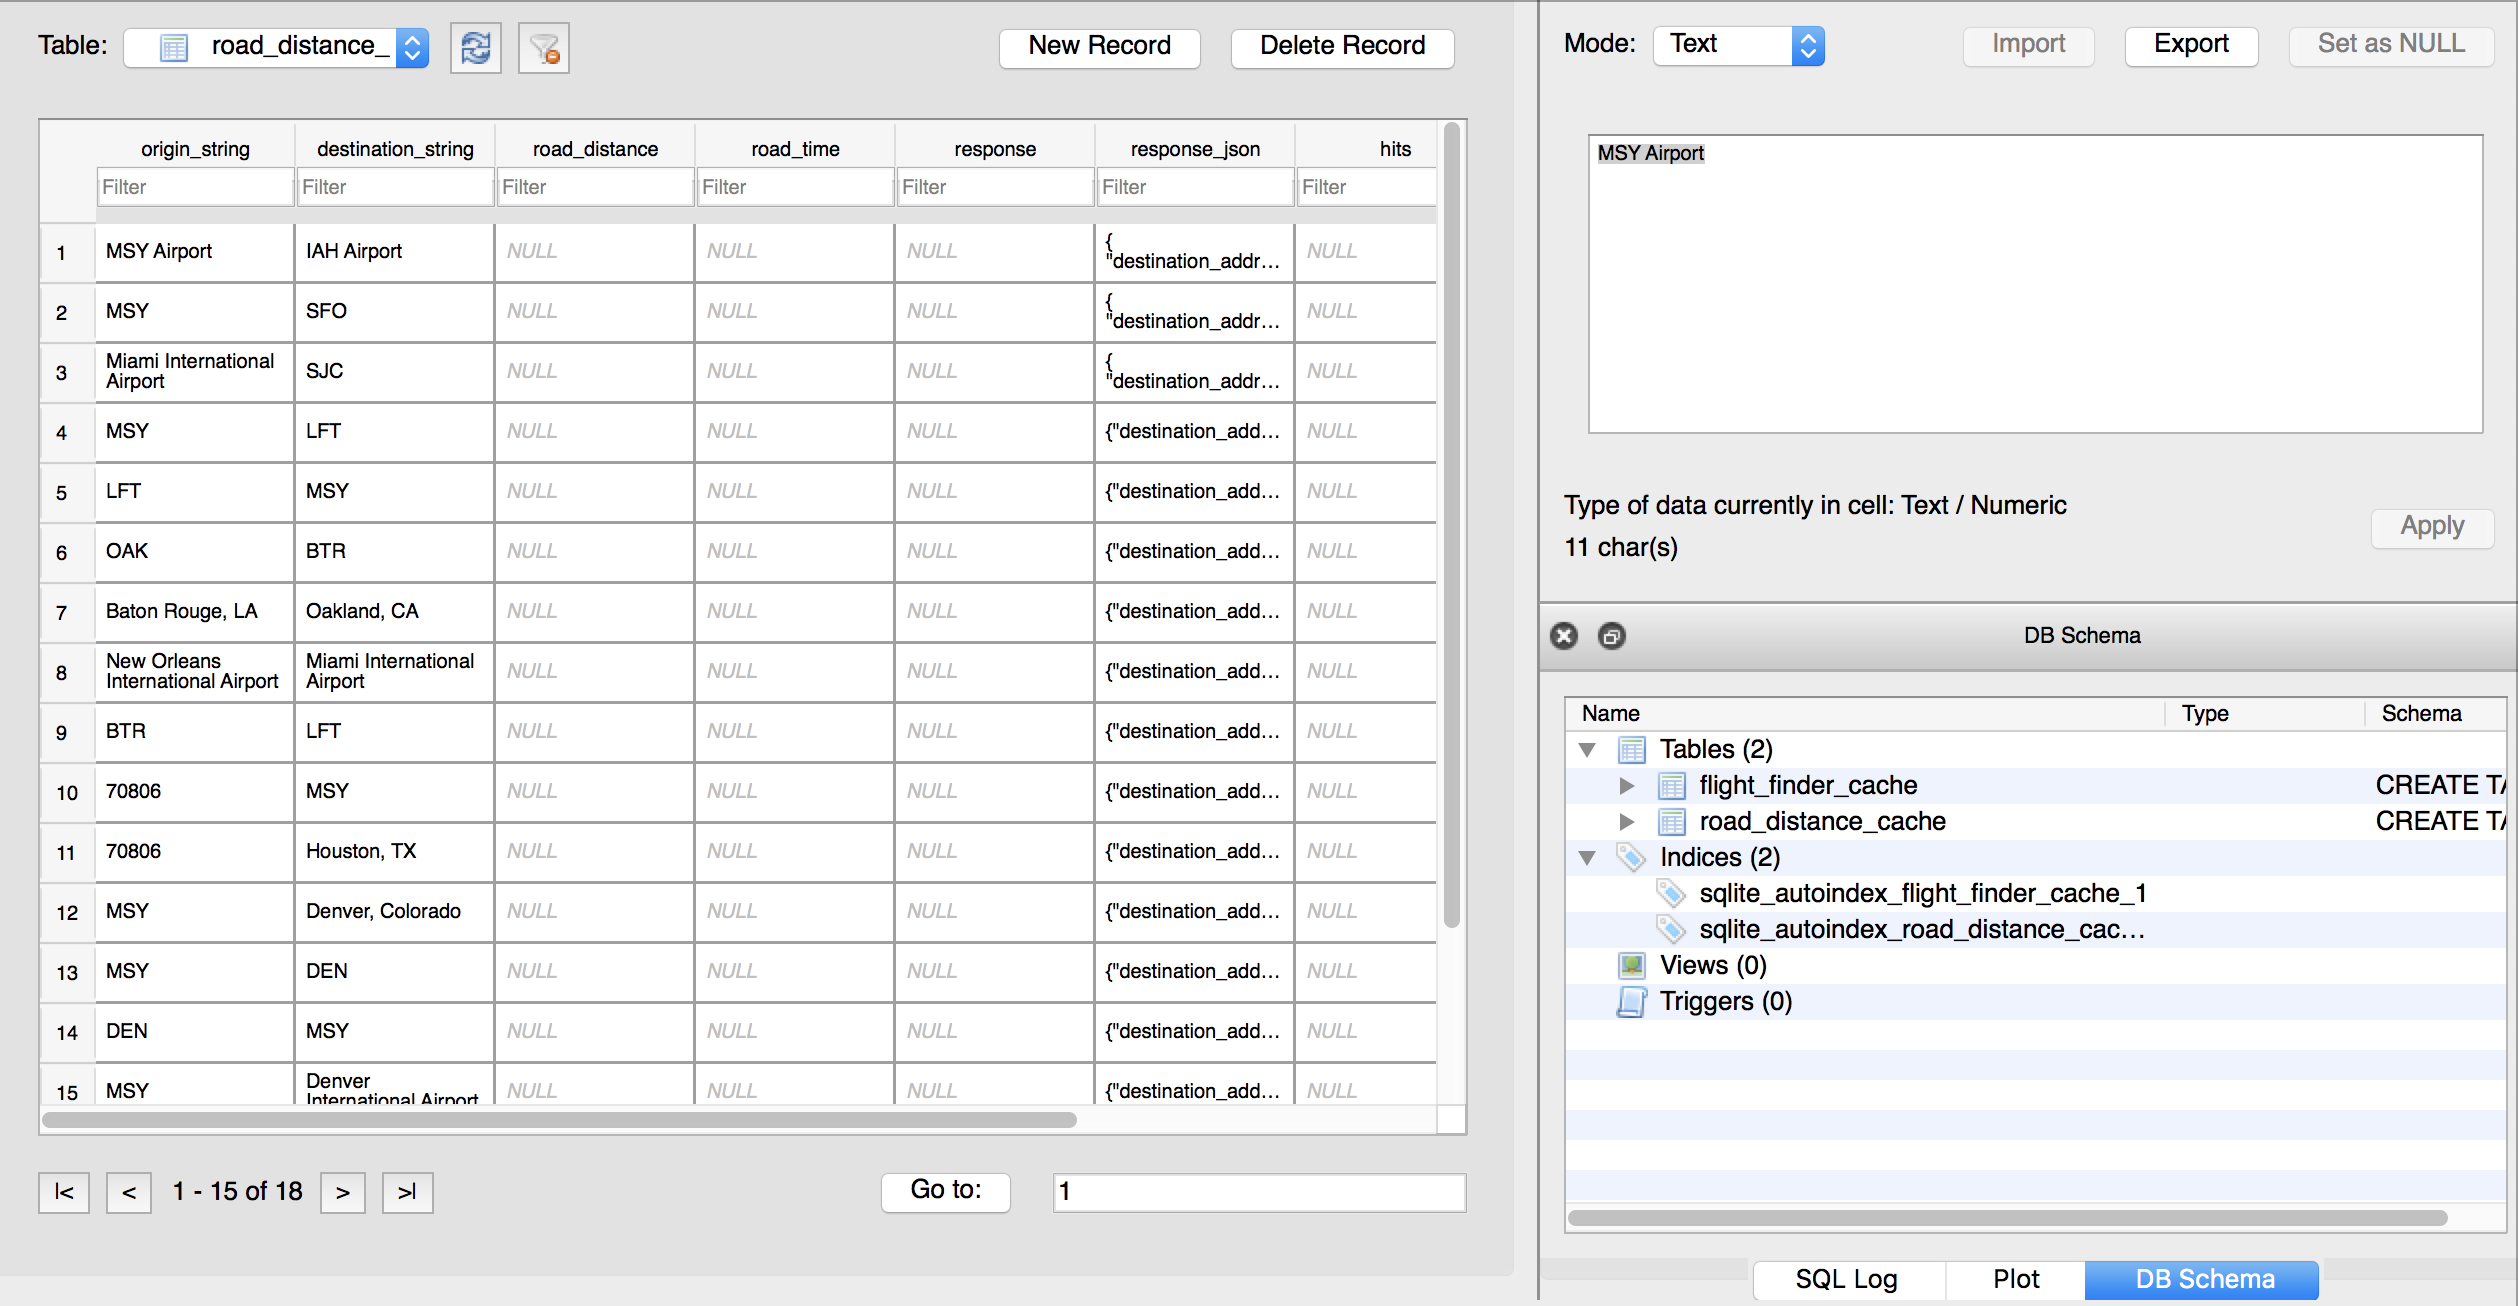
\includegraphics[width=0.9\textwidth]{db}
  \caption{SQLite database}
  \label{fig:db}
\end{figure}

\section{Future Work}
This application is restricted to traveling within the US. Other countries could be included to give the user the option to travel internationally. The only modes of transportation that are used are driving and flying. To give the user a more flexibility when traveling, other modes of transportation could be incorporated into this application such as walking, bicycling, taking the train or metro, and taking a ferry.

Additionally, after caching of a large amount of data our application could make certain predictions which improve our search algorithm.  For example, instead of choosing the $n$ nearest airports to add to our search tree, Watson Analytics predict feature could also choose an airport which may be slightly farther away but which may frequently have deals on flights.
				

\end{document}
